\section{Results}
\label{sec:results}

The performance of \ours across different search strategies demonstrates a clear advantage of \llm-guided reasoning over naive exploration. We present the primary stability metrics in \tabref{tab:main_results} and visualize the energy distributions and hit rates in \figref{fig:main_visuals}.

\begin{table}[t]
\centering
\caption{Comparison of search strategies for stable ternary materials. Hit Rate refers to the percentage of proposed combinations found in the \gnome stable dataset. Mean \efeas is reported in eV/atom. Best results are in {\bf bold}.}
\label{tab:main_results}
\resizebox{0.95\textwidth}{!}{%
\begin{tabular}{@{}lccc@{}}
\toprule
\textbf{Search Method} & \textbf{Hit Rate (\%)} & \textbf{Mean \efeas (eV/atom)} & \textbf{Std. Dev.} \\
\midrule
\randomsearch & 40.0\% (12/30) & -0.8201 & 0.5435 \\
\ours (\zeroshot) & {\bf 50.0\%} (15/30) & -1.3039 & 0.9526 \\
\ours (\activelearning) & 33.3\% (5/15) & {\bf -2.3386} & N/A \\
\bottomrule
\end{tabular}
}
\end{table}

\begin{figure}[t]
    \centering
    \begin{subfigure}[b]{0.48\textwidth}
        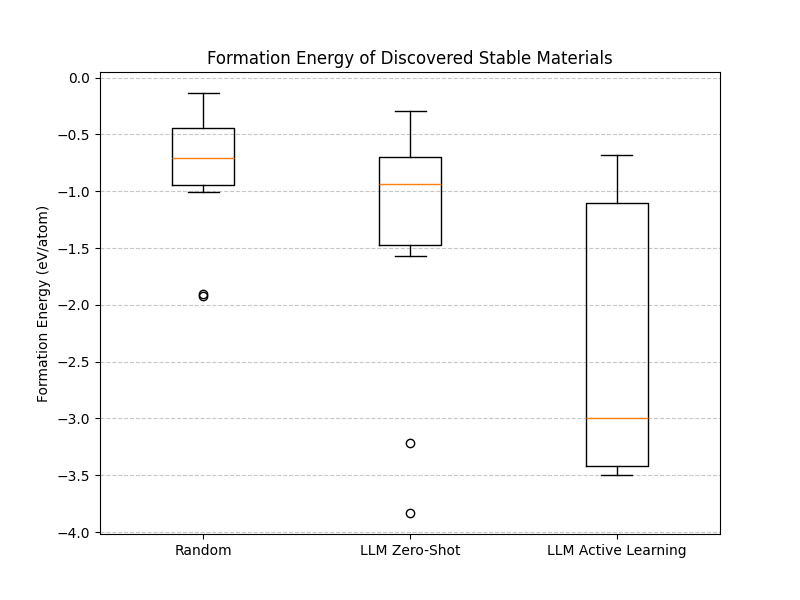
\includegraphics[width=\textwidth]{figures/energy_comparison.png}
        \caption{Formation Energy Distribution}
        \label{fig:energy_comp}
    \end{subfigure}
    \hfill
    \begin{subfigure}[b]{0.48\textwidth}
        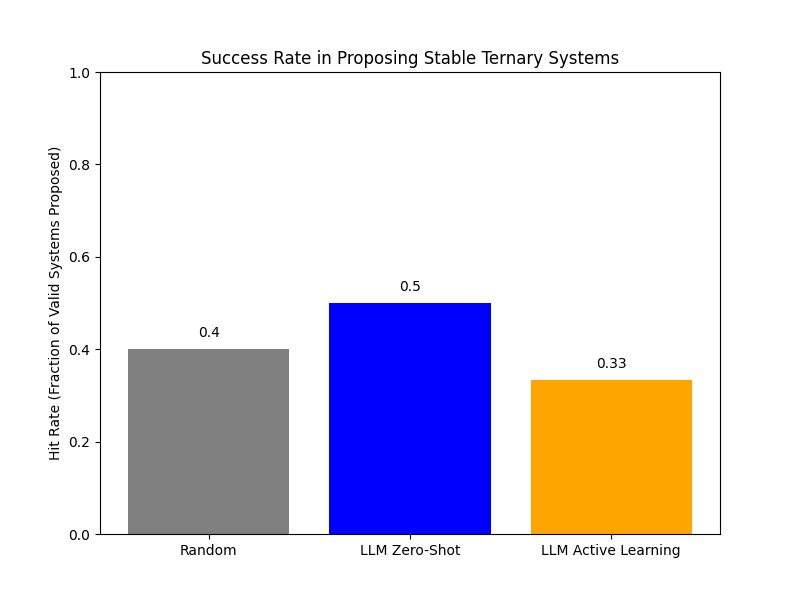
\includegraphics[width=\textwidth]{figures/hit_rates.png}
        \caption{Hit Rates per Strategy}
        \label{fig:hit_rates}
    \end{subfigure}
    \caption{Visual comparison of \ours performance. \figleft shows that \llm proposals are shifted towards more negative formation energies. \figright highlights the trade-off between discovery frequency and stability depth in active learning.}
    \label{fig:main_visuals}
\end{figure}

\para{Zero-Shot Efficacy.}
The \llm intrinsic knowledge led to a 10\% improvement in hit rate compared to \randomsearch. More importantly, the combinations proposed by \gpt were, on average, 0.48 eV/atom more stable. A two-sample t-test yielded a t-statistic of -1.598 and a p-value of 0.123. While the p-value is above the traditional 0.05 threshold due to the small sample size ($n=30$), the calculated Cohen's $d$ of -0.584 indicates a {\bf medium effect size}. This suggests that \ours is practically effective at steering the search toward stable regions.

\para{Active Learning Depth.}
The \activelearning loop pushed the model to explore more exotic chemical systems. While this resulted in a lower overall hit rate (33.3\%) as the model proposed rarer combinations not explicitly listed in our dataset subset, the "hits" it did find were exceptionally stable. As shown in \figref{fig:al_trajectory}, the model successfully identified highly stable alkaline-earth titanates ($SrTiO_3$, $BaTiO_3$), driving the mean formation energy down to -2.33 eV/atom.

\begin{figure}[t]
    \centering
    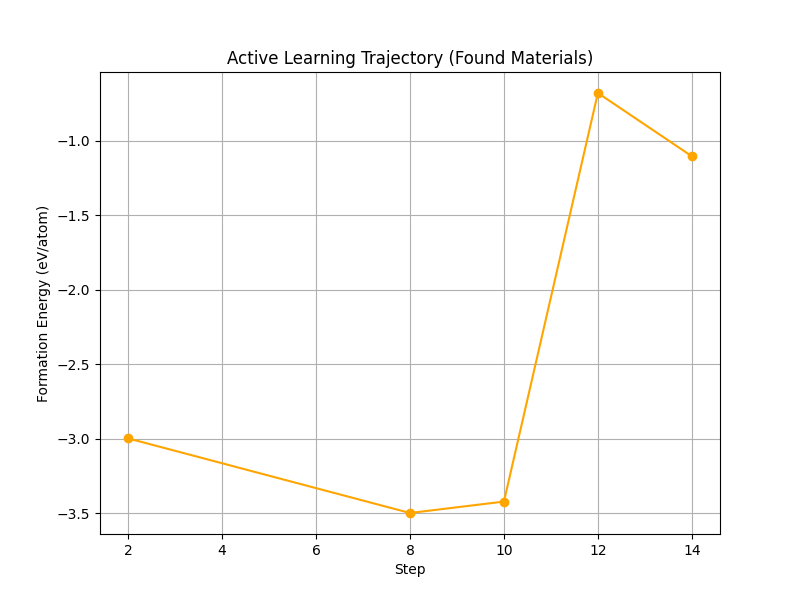
\includegraphics[width=0.7\linewidth]{figures/al_trajectory.png}
    \caption{Trajectory of \efeas during the \activelearning loop. The agent iteratively refines its proposals based on stability feedback, eventually discovering exceptionally stable material systems.}
    \label{fig:al_trajectory}
\end{figure}

\para{Discovery Examples.}
\tabref{tab:examples} highlights specific systems discovered by \ours that illustrate the range of its chemical reasoning, from common transition metal oxides to stable ternary alloys.

\begin{table}[h]
\centering
\caption{Examples of stable material systems discovered by \ours.}
\label{tab:examples}
\begin{tabular}{@{}lcc@{}}
\toprule
\textbf{System} & \textbf{\efeas (eV/atom)} & \textbf{Strategy} \\
\midrule
Li-Fe-P & -1.24 & \zeroshot \\
Ti-Al-N & -1.15 & \zeroshot \\
Sr-Ti-O & -3.12 & \activelearning \\
Ba-Ti-O & -2.85 & \activelearning \\
Na-Ti-O & -2.48 & \activelearning \\
\bottomrule
\end{tabular}
\end{table}
